\documentclass{beamer}
\usepackage{graphicx}
\usepackage{xcolor}
\usepackage{tikz}
\usepackage{amsmath}
\DeclareGraphicsExtensions{.png,.pdf,.jpg,.jpeg}

\definecolor{purpleblue}{RGB}{80, 80, 180}
\definecolor{lightgray}{RGB}{230, 230, 230}
\definecolor{novelPurple}{RGB}{98, 54, 255}
\definecolor{darkgray}{RGB}{50, 50, 50}
\definecolor{softPurple}{RGB}{180, 170, 255}
\definecolor{softGray}{RGB}{235, 235, 245}
\definecolor{lightText}{RGB}{90, 90, 110}
\graphicspath{{static/unit4/}{./}}

\usetheme{Madrid}
\usecolortheme{dolphin}

\setbeamerfont{title}{size=\Large,series=\bfseries}
\setbeamerfont{frametitle}{size=\LARGE,series=\bfseries}
\setbeamercolor{frametitle}{fg=white, bg=novelPurple}
\setbeamercolor{title}{fg=white, bg=purpleblue}

\title[SAT Unit 4.2]{\textbf{SAT Unit 4.2 \\Lines, Angles, and Triangles}}
\author{\textbf{Jack Zeng}}
\institute{\textcolor{white}{\textbf{Novel Prep}}}
\date{\today}

\begin{document}

\begin{frame}
    \titlepage
    \vfill
    \begin{flushright}
        \textcolor{purpleblue}{\Huge \textbf{Novel Prep}}
    \end{flushright}
\end{frame}

\begin{frame}
    \begin{tikzpicture}[remember picture, overlay]
        \shade[top color=softPurple, bottom color=softGray]
            (current page.north west) rectangle (current page.south east);
        \fill[white, opacity=0.3] (current page.center) circle (4cm);
        \node[align=center] at (current page.center) {
            {\Huge\bfseries\textcolor{purpleblue}{Novel Prep}} \\[0.5cm]
            {\Large\itshape\textcolor{lightText}{Excellence in SAT Prep}}
        };
        \foreach \x in {1,2,3,4,5} {
            \fill[purpleblue, opacity=0.2] (rand*10-5, rand*7-3.5) circle (0.1+\x*0.05);
        }
    \end{tikzpicture}
\end{frame}

\begin{frame}{Overview}
    \tableofcontents
\end{frame}


\begin{frame}
\section{Line}
    \begin{tikzpicture}[remember picture, overlay]
        \shade[top color=softPurple, bottom color=softGray]
            (current page.north west) rectangle (current page.south east);
        \fill[white, opacity=0.3] (current page.center) circle (4cm);
        \node[align=center] at (current page.center) {
            {\LARGE\bfseries\textcolor{purpleblue}{Line}} \\[0.5cm]
            {\Large\itshape\textcolor{lightText}{Excellence in SAT Prep}}
        };
        \foreach \x in {1,2,3,4,5} {
            \fill[purpleblue, opacity=0.2] (rand*10-5, rand*7-3.5) circle (0.1+\x*0.05);
        }
    \end{tikzpicture}
\end{frame}


\begin{frame}{Definition of Line, Segment, and Ray}
\begin{itemize}
    \item \textbf{Line:} a straight arrangement of points extending infinitely in both directions.
    \item \textbf{Segment:} part of a line with two endpoints.
    \item \textbf{Ray:} part of a line with one endpoint extending infinitely in one direction.
\end{itemize}
\end{frame}

\begin{frame}
\section{Angle}
    \begin{tikzpicture}[remember picture, overlay]
        \shade[top color=softPurple, bottom color=softGray]
            (current page.north west) rectangle (current page.south east);
        \fill[white, opacity=0.3] (current page.center) circle (4cm);
        \node[align=center] at (current page.center) {
            {\LARGE\bfseries\textcolor{purpleblue}{Angle}} \\[0.5cm]
            {\Large\itshape\textcolor{lightText}{Excellence in SAT Prep}}
        };
        \foreach \x in {1,2,3,4,5} {
            \fill[purpleblue, opacity=0.2] (rand*10-5, rand*7-3.5) circle (0.1+\x*0.05);
        }
    \end{tikzpicture}
\end{frame}


\begin{frame}{Angle Relationships}

\begin{itemize}
    \item Vertical angles are equal.
    \item A linear pair sums to $180^\circ$.
    \item Angles around a point sum to $360^\circ$.
\end{itemize}

\vspace{0.2cm}
\textbf{SAT move:} mark what you know on the diagram first, then chase missing angles one relationship at a time.

\end{frame}

\begin{frame}{Parallel Lines and Transversals}

When two parallel lines are cut by a transversal:
\begin{itemize}
    \item Corresponding angles are equal.
    \item Alternate interior angles are equal.
    \item Same-side interior angles sum to $180^\circ$.
\end{itemize}

\vspace{0.2cm}
\textbf{Shortcut:} if you see arrow marks for parallel lines, immediately look for equal or supplementary angle pairs.

\end{frame}

\begin{frame}
\section{Triangle}
    \begin{tikzpicture}[remember picture, overlay]
        \shade[top color=softPurple, bottom color=softGray]
            (current page.north west) rectangle (current page.south east);
        \fill[white, opacity=0.3] (current page.center) circle (4cm);
        \node[align=center] at (current page.center) {
            {\LARGE\bfseries\textcolor{purpleblue}{Triangle}} \\[0.5cm]
            {\Large\itshape\textcolor{lightText}{Excellence in SAT Prep}}
        };
        \foreach \x in {1,2,3,4,5} {
            \fill[purpleblue, opacity=0.2] (rand*10-5, rand*7-3.5) circle (0.1+\x*0.05);
        }
    \end{tikzpicture}
\end{frame}


\begin{frame}{Triangles: Core Facts}

\begin{itemize}
    \item Interior angles of a triangle sum to $180^\circ$.
    \item Exterior angle equals the sum of the two remote interior angles.
    \item Isosceles triangle: equal sides have equal opposite angles.
    \item Triangle area: $A=\dfrac{1}{2}bh$.
\end{itemize}

\end{frame}

\begin{frame}{Triangle Congruence}

\textbf{Common congruence reasons:}
\begin{itemize}
    \item SSS: three sides match
    \item SAS: two sides and included angle match
    \item ASA/AAS: two angles and one side match
    \item HL: right triangles with hypotenuse and one leg match
\end{itemize}

\vspace{0.2cm}
\textbf{After congruence:} corresponding sides and angles are equal (CPCTC).

\end{frame}

\begin{frame}{Similar Triangles}

\textbf{AA similarity:} two equal angles are enough.

\vspace{0.2cm}
For similar triangles:
\[
\dfrac{\text{side}_1}{\text{matching side}_1}
=
\dfrac{\text{side}_2}{\text{matching side}_2}
\]

\vspace{0.2cm}
\textbf{SAT move:} write the proportion using matching positions, not just visually close sides.

\end{frame}

\begin{frame}{Coordinate Geometry With Triangles}

\begin{itemize}
    \item Horizontal/vertical distances can be read from coordinates.
    \item Distance formula: $d=\sqrt{(x_2-x_1)^2+(y_2-y_1)^2}$.
    \item Slope helps identify parallel or perpendicular lines.
    \item Area can be found by enclosing the triangle in a rectangle and subtracting.
\end{itemize}

\end{frame}

\begin{frame}{Worked Example: Triangle Area}

\textbf{Question:} A triangle has base $18$ and height $7$. What is its area?

\vspace{0.2cm}
\[
A=\dfrac{1}{2}bh=\dfrac{1}{2}(18)(7)=63
\]

\textbf{Answer:} $\boxed{63}$.

\end{frame}

\begin{frame}
\section{Practice}
    \begin{tikzpicture}[remember picture, overlay]
        \shade[top color=softPurple, bottom color=softGray]
            (current page.north west) rectangle (current page.south east);
        \fill[white, opacity=0.3] (current page.center) circle (4cm);
        \node[align=center] at (current page.center) {
            {\LARGE\bfseries\textcolor{purpleblue}{Practice}} \\[0.5cm]
            {\Large\itshape\textcolor{lightText}{Excellence in SAT Prep}}
        };
        \foreach \x in {1,2,3,4,5} {
            \fill[purpleblue, opacity=0.2] (rand*10-5, rand*7-3.5) circle (0.1+\x*0.05);
        }
    \end{tikzpicture}
\end{frame}

\begin{frame}{Question: In the figure, AC = CD. The measure of angle EBC is 45°, and the measure…}
\begin{center}
    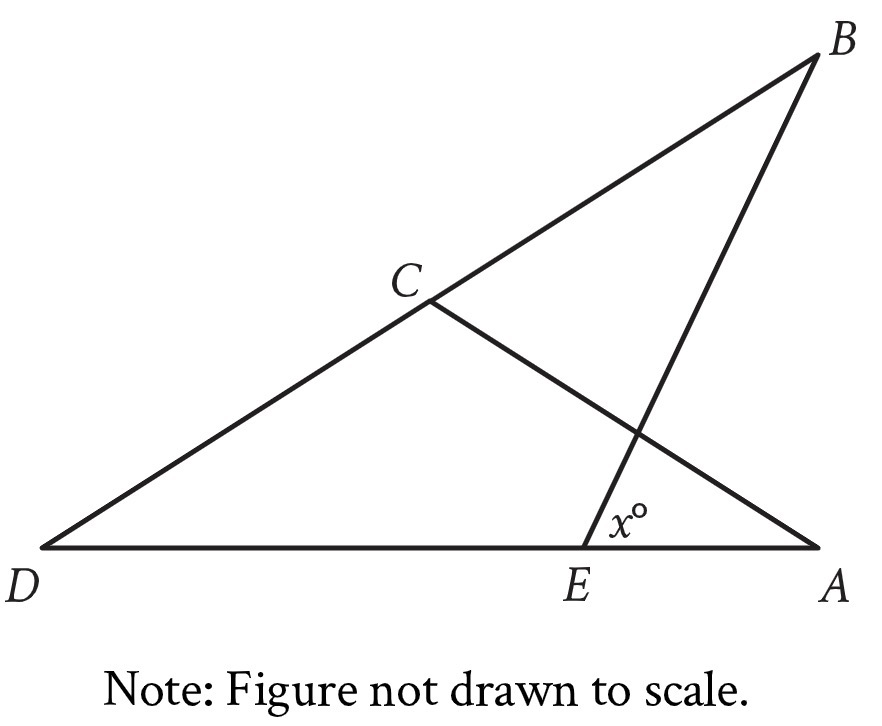
\includegraphics[width=0.54\linewidth]{7.jpg}
\end{center}

\textbf{In the figure, $AC = CD$. The measure of angle $\angle EBC$ is $45^\circ$, and the measure of angle $\angle ACD$ is $104^\circ$. What is the value of $x$?}
\end{frame}
\begin{frame}{Answer: In the figure, AC = CD. The measure of angle EBC is 45°, and the measure…}
\textit{Strategy:} Isosceles sides $AC=CD$; use triangle angle sum and exterior angles.

\textbf{Solution:}
\[ \boxed{83} \]
\textbf{Correct Answer:} \( \boxed{83} \)

\end{frame}
\begin{frame}{Question: In the figure shown, points Q, R, S, and T lie on line segment PV, and l…}
\begin{center}
    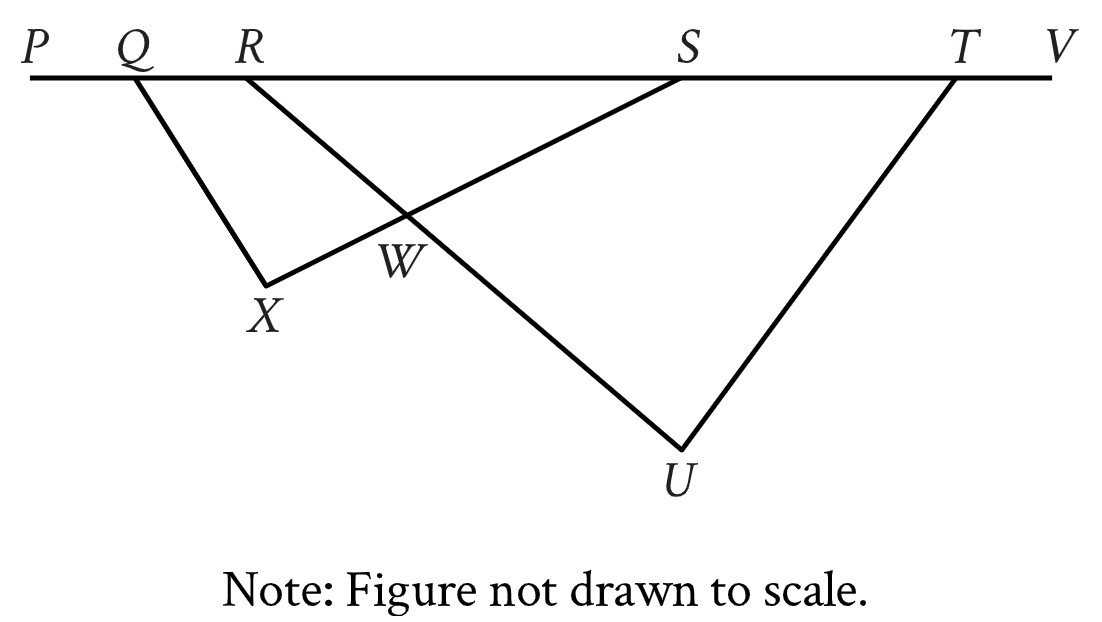
\includegraphics[width=0.62\linewidth]{8.jpg}
\end{center}

In the figure shown, points $Q$, $R$, $S$, and $T$ lie on line segment $\overline{PV}$, and line segment $\overline{RU}$ intersects line segment $\overline{SX}$ at point $W$.  
The measure of $\angle SQX$ is $48^\circ$, the measure of $\angle SXQ$ is $86^\circ$, the measure of $\angle SWU$ is $85^\circ$, and the measure of $\angle VTU$ is $162^\circ$.  
What is the measure, in degrees, of $\angle TUR$?
\end{frame}
\begin{frame}{Answer: In the figure shown, points Q, R, S, and T lie on line segment PV, and l…}
\textit{Strategy:} Track angles around point $W$ using triangle sum and linear pairs.

\textbf{Solution:}
\[ \boxed{123} \]
\textbf{Correct Answer:} \( \boxed{123} \)

\end{frame}
\begin{frame}{Question: Intersecting lines r, s, and t are shown below}
\begin{center}
    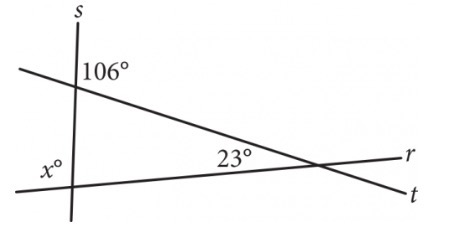
\includegraphics[width=0.54\linewidth]{9.jpg}
\end{center}

Intersecting lines $r$, $s$, and $t$ are shown below.  
What is the value of $x$?
\end{frame}
\begin{frame}{Answer: Intersecting lines r, s, and t are shown below}
\textit{Strategy:} Three intersecting lines: vertical and supplementary angle pairs.

\textbf{Solution:}
\[ \boxed{97} \]
\textbf{Correct Answer:} \( \boxed{97} \)

\end{frame}
\begin{frame}{Question: In the figure above, MQ and NR intersect at point P, NP = QP, and MP = P…}
\begin{center}
    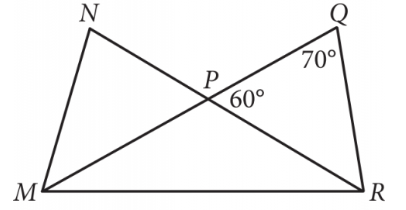
\includegraphics[width=0.54\linewidth]{10.png}
\end{center}

In the figure above, $\overline{MQ}$ and $\overline{NR}$ intersect at point $P$, $NP = QP$, and $MP = PR$.  
What is the measure, in degrees, of $\angle QMR$? (Disregard the degree symbol when gridding your answer.)
\end{frame}
\begin{frame}{Answer: In the figure above, MQ and NR intersect at point P, NP = QP, and MP = P…}
\textit{Strategy:} Vertical angles and linear pairs at intersection $Q$.

\textbf{Solution:}
\[ \boxed{30} \]
\textbf{Correct Answer:} \( \boxed{30} \)

\end{frame}
\begin{frame}{Question: In triangle ABC, the measure of angle B is 90° and BD is an altitude of …}
In triangle $ABC$, the measure of angle $B$ is $90^\circ$ and $\overline{BD}$ is an altitude of the triangle.  
The length of $\overline{AB}$ is $15$ and the length of $\overline{AC}$ is $23$ greater than the length of $\overline{AB}$.  
What is the value of $\dfrac{BC}{BD}$?
\begin{itemize}
    \item[\textbf{A.}] $\dfrac{15}{38}$
    \item[\textbf{B.}] $\dfrac{15}{23}$
    \item[\textbf{C.}] $\dfrac{23}{15}$
    \item[\textbf{D.}] $\dfrac{38}{15}$
\end{itemize}
\end{frame}
\begin{frame}{Answer: In triangle ABC, the measure of angle B is 90° and BD is an altitude of …}
\textit{Strategy:} Parallel lines + transversal: alternate interior angles are equal.

\textbf{Correct Answer:} \( \boxed{D} \)

\end{frame}
\begin{frame}{Question: In triangles ABC and DEF, angles B and E each have measure 27° and angle…}
In triangles $ABC$ and $DEF$, angles $B$ and $E$ each have measure $27^\circ$ and angles $C$ and $F$ each have measure $41^\circ$.  
Which additional piece of information is sufficient to determine whether triangle $ABC$ is congruent to triangle $DEF$?
\begin{itemize}
    \item[\textbf{A.}] The measure of angle $A$
    \item[\textbf{B.}] The length of side $\overline{AB}$
    \item[\textbf{C.}] The lengths of sides $\overline{BC}$ and $\overline{EF}$
    \item[\textbf{D.}] No additional information is necessary.
\end{itemize}
\end{frame}
\begin{frame}{Answer: In triangles ABC and DEF, angles B and E each have measure 27° and angle…}
\textit{Strategy:} Triangle sum is $180^\circ$; combine with isosceles base angles.

\textbf{Correct Answer:} \( \boxed{C} \)

\end{frame}
\begin{frame}{Question: In triangles LMN and RST, angles L and R each have measure 60°, LN = 10,…}
In triangles $LMN$ and $RST$, angles $L$ and $R$ each have measure $60^\circ$, $\overline{LN} = 10$, and $\overline{RT} = 30$.  
Which additional piece of information is sufficient to prove that triangle $LMN$ is similar to triangle $RST$?
\begin{itemize}
    \item[\textbf{A.}] $\overline{MN} = 7$ and $\overline{ST} = 7$
    \item[\textbf{B.}] $\overline{MN} = 7$ and $\overline{ST} = 21$
    \item[\textbf{C.}] The measures of angles $M$ and $S$ are $70^\circ$ and $60^\circ$, respectively.
    \item[\textbf{D.}] The measures of angles $M$ and $T$ are $70^\circ$ and $50^\circ$, respectively.
\end{itemize}
\end{frame}
\begin{frame}{Answer: In triangles LMN and RST, angles L and R each have measure 60°, LN = 10,…}
\textit{Strategy:} Exterior angle equals sum of remote interior angles.

\textbf{Correct Answer:} \( \boxed{D} \)

\end{frame}
\begin{frame}{Question: In the figure above, what is the length of NQ?}
\begin{center}
    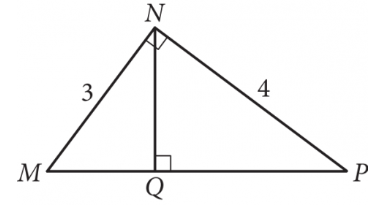
\includegraphics[width=0.54\linewidth]{11.png}
\end{center}

In the figure above, what is the length of $\overline{NQ}$?
\begin{itemize}
    \item[\textbf{A.}] $2.2$
    \item[\textbf{B.}] $2.3$
    \item[\textbf{C.}] $2.4$
    \item[\textbf{D.}] $2.5$
\end{itemize}
\end{frame}
\begin{frame}{Answer: In the figure above, what is the length of NQ?}
\textit{Strategy:} Congruent triangles: match corresponding parts (CPCTC).

\textbf{Correct Answer:} \( \boxed{C} \)

\end{frame}
\begin{frame}{Question: Triangle XYZ is similar to triangle RST such that X, Y, and Z correspond…}
Triangle $XYZ$ is similar to triangle $RST$ such that $X, Y,$ and $Z$ correspond to $R, S,$ and $T$, respectively.  
The measure of $\angle Z$ is $20^\circ$ and $2\overline{XY} = \overline{RS}$.  
What is the measure of $\angle T$?
\begin{itemize}
    \item[\textbf{A.}] $2^\circ$
    \item[\textbf{B.}] $10^\circ$
    \item[\textbf{C.}] $20^\circ$
    \item[\textbf{D.}] $40^\circ$
\end{itemize}
\end{frame}
\begin{frame}{Answer: Triangle XYZ is similar to triangle RST such that X, Y, and Z correspond…}
\textit{Strategy:} Similar triangles: set up a proportion for missing length.

\textbf{Correct Answer:} \( \boxed{C} \)

\end{frame}
\begin{frame}{Question: In the figure above, RT = TU}
\begin{center}
    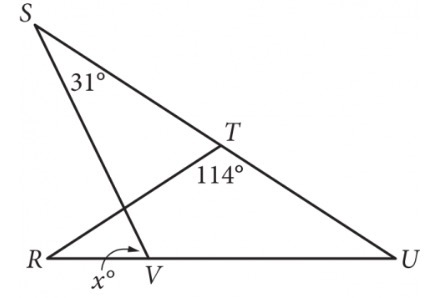
\includegraphics[width=0.54\linewidth]{12.jpg}
\end{center}

In the figure above, $\overline{RT} = \overline{TU}$.  
What is the value of $x$?
\begin{itemize}
    \item[\textbf{A.}] $72$
    \item[\textbf{B.}] $66$
    \item[\textbf{C.}] $64$
    \item[\textbf{D.}] $58$
\end{itemize}
\end{frame}
\begin{frame}{Answer: In the figure above, RT = TU}
\textit{Strategy:} Area ratio of similar triangles equals $(\text{scale factor})^2$.

\textbf{Correct Answer:} \( \boxed{C} \)

\end{frame}
\begin{frame}{Question: The area of triangle ABC above is at least 48 but no more than 60. If y …}
\begin{center}
    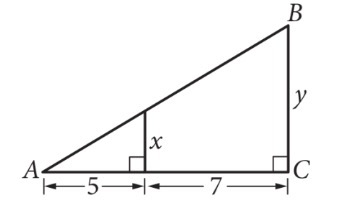
\includegraphics[width=0.54\linewidth]{13.jpg}
\end{center}

The area of triangle $ABC$ above is at least $48$ but no more than $60$. If $y$ is an integer, what is one possible value of $x$?
\end{frame}
\begin{frame}{Answer: The area of triangle ABC above is at least 48 but no more than 60. If y …}
\textit{Strategy:} Coordinate geometry: slope or distance for parallel/perpendicular.

\textbf{Solution:}
\[ \boxed{10/3} \]
\textit{Also accept: 15/4, 25/6}
\textbf{Correct Answer:} \( \boxed{10/3} \)

\end{frame}
\begin{frame}{Question: In triangle RST, angle T is a right angle, point L lies on RS, point K l…}
In triangle $RST$, angle $T$ is a right angle, point $L$ lies on $\overline{RS}$, point $K$ lies on $\overline{ST}$, and $\overline{LK}$ is parallel to $\overline{RT}$.  
If the length of $\overline{RT}$ is $72$ units, the length of $\overline{LK}$ is $24$ units, and the area of triangle $RST$ is $792$ square units, what is the length of $\overline{KT}$, in units?
\end{frame}
\begin{frame}{Answer: In triangle RST, angle T is a right angle, point L lies on RS, point K l…}
\textit{Strategy:} Angle chase using straight angle ($180^\circ$) and vertical angles.

\textbf{Solution:}
\[ \boxed{14.66} \]
\textit{Also accept: 14.67, 44/3}
\textbf{Correct Answer:} \( \boxed{14.66} \)

\end{frame}
\begin{frame}{Question: In the figure, parallel lines q and t are intersected by lines r and s}
\begin{center}
    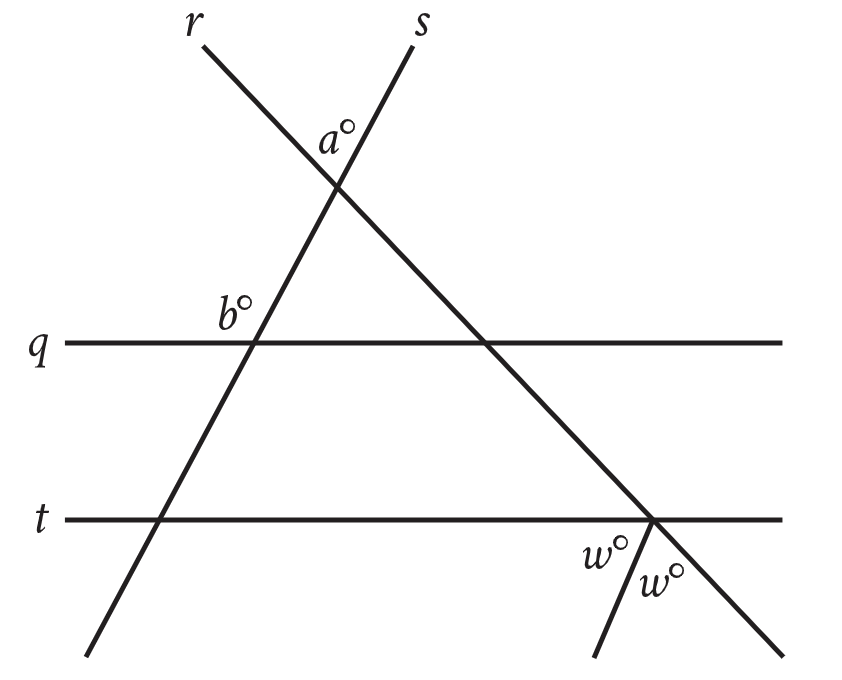
\includegraphics[width=0.54\linewidth]{14.png}
\end{center}

In the figure, parallel lines $q$ and $t$ are intersected by lines $r$ and $s$.  
If $a = 43^\circ$ and $b = 122^\circ$, what is the value of $w$?
\end{frame}
\begin{frame}{Answer: In the figure, parallel lines q and t are intersected by lines r and s}
\textit{Strategy:} ASA/AAS/SAS: identify which congruence criterion applies.

\textbf{Solution:}
\[ \boxed{101/2} \]
\textit{Also accept: 50.5}
\textbf{Correct Answer:} \( \boxed{101/2} \)

\end{frame}
\begin{frame}{Question: In the figure above, BD = 6 and AD = 8}
\begin{center}
    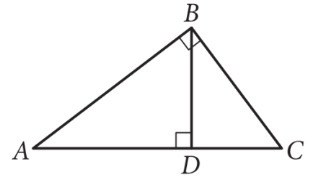
\includegraphics[width=0.54\linewidth]{16.jpg}
\end{center}

In the figure above, $\overline{BD} = 6$ and $\overline{AD} = 8$.  
What is the length of $\overline{DC}$?
\end{frame}
\begin{frame}{Answer: In the figure above, BD = 6 and AD = 8}
\textit{Strategy:} Use $\dfrac{1}{2}bh$ after finding base and height from the diagram.

\textbf{Solution:}
\[ \boxed{4.5} \]
\textbf{Correct Answer:} \( \boxed{4.5} \)

\end{frame}

\begin{frame}{}
    \begin{tikzpicture}[remember picture, overlay]
        \shade[top color=novelPurple!40, bottom color=white]
            (current page.north west) rectangle (current page.south east);
        \fill[white, opacity=0.15] (current page.center) circle (5cm);
        \foreach \x in {1,2,3,4,5} {
            \fill[novelPurple, opacity=0.12] (rand*10-5, rand*7-3.5) circle (0.1+\x*0.05);
        }
    \end{tikzpicture}
    \centering
    \vspace{5em}
    {\Huge \textbf{\textcolor{novelPurple}{Thank You!}}} \\[1em]
    {\large \textcolor{gray}{We appreciate your time and focus.}} \\[3em]
    {\LARGE \textbf{\textcolor{novelPurple}{\textsf{Novel Prep}}}}
    \vfill
\end{frame}

\end{document}
